\section{Lucene}


Lucene jest biblioteką napisaną w Javie. Biblioteka ta jest w stanie indeksować dużą ilość dokumentów z różnych źródeł i przeprowadzać szybkie wyszukiwania w tych tekstach. W opisywanej aplikacji, framework Lucene przechowuje źródła stron. Strony te zostały pobrane z  serwisu delicous i zapisane w bazie danych. 

\subsection{Pobieranie stron}

W pewnych odstępach czasu, wątek odpowiedzialny za indeksowanie stron sprawdza czy w bazie danych tabela DOCUMENT nie ma informacji o nowych wpisach. Z bazy danych pobrane są informacje o adresach tych stron. Następnie dla każdego adresu URL zostaje pobrana treść strony na którą wskazuje. Strona WWW następnie zostaje oczyszczona ze znaczników HTML, i przekazane do frameworku lucene do zindeksowania. Jeśli wszystkie czynności zakończą się powodzeniem, w bazie danych zostaje odnotowana informacja o posiadaniu na dysku danego dokumentu. Rysunek \ref{fig:lucene_index_fig} przedstawiony jest cały proces pobierania i przetwarzania danej strony.

\begin{figure}[htb]

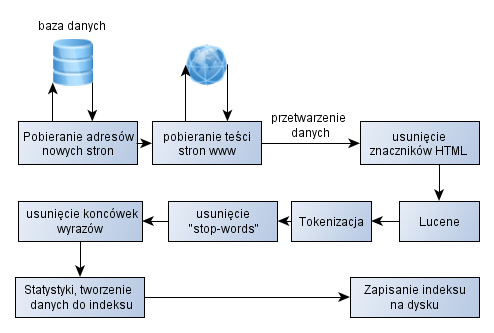
\includegraphics[width=1\textwidth]{lucene_indeksing.png}
\caption{Lucene: pobieranie danych i indeksowanie}
\label{fig:lucene_index_fig}
\end{figure}

Do Lucene zapisywane są następujące informacje: identyfikator $id$ dokumentu z bazy danych, oraz przetworzony tekst strony WWW. Przechowywanie identyfikatora dokumentu w danych Lucene pozwala późniejsze powiązanie wyników wyszukiwania z odpowiednim rekordem w bazie danych. 

W czasie indeksowania biblioteka Lucene wykonuje wiele czynności które pozwalają jej później szybko wyszukiwać informację. Główne z nich to:
\begin{itemize}
\item Tekst zostanie przetworzony na ciąg termów,
\item usunięcie końcówek wyrazów,
\item usunięcie 'stop-words' z tekstu, czyli słów nie mających dużego znaczenia przy wynikach wyszukiwania, takich jak: i, lub, ...
\item obliczenie statystyk, np: wystąpienia słów w dokumencie, odległości od siebie
\end{itemize}


Czas wyszukiwania zapytania w dokumentach przechowywanych Lucene jest szybkie. Przy małej, poniżej 1GB danych, wyszukiwanie następuje praktycznie w czasie rzeczywistym. Zapytanie jest przekazywane do frameworku, w którym jest one przekształcane na termy. Dla zapytania $q$ i dla każdego dokumentu $d$ wyliczana jest wartość funkcji $score(q,d)$. Wynikiem są dokumenty posortowane wg. wyniku tej funkcji.

$score(q,d) =   coord(q,d)  *  queryNorm(q) * \sum_{t \text{ in } q}  \bigg( tf(t\text{ in } d)  *  idf(t)^2  *  getBoost(t) *  norm(t,d) )$

gdzie:
\begin{itemize}
	\item coord(q,d): funkcja zwraca wartości zależne od miejsca występowania i odległości od siebie szukanych termów w dokumencie.
	\item queryNorm(q): funkcja normalizująca wyniki zapytania
	\item tf(t in d): funkcja wyliczająca częstość występowania danego termu w dokumencie
	\item idf(t) : funkcja wyliczająca częstość występowania termu we wszystkich dokumentach.
	\item getBoost(t) - Lucene pozwala na zwiększenie wagi niektórych termów. Nieużywane w tej aplikacji.
\end{itemize}

Lucene ocenia dokumenty głównie na podstawie funkcji TF-IDF. Każdy dokument reprezentowany jest przez wektor, składający się z wag słów występujących w tym dokumencie. TFIDF informuje o częstości wystąpienia termów uwzględniając jednocześnie odpowiednie wyważenie znaczenia lokalnego termu i jego znaczenia w kontekście pełnej kolekcji dokumentów.
